\chapter{Development Process}\label{chap:developmentprocess}

\textcolor{orange}{NOE TEKST}

\section{Code Repositories}

% Github Organization and repos
All code and project-related resources are stored on GitHub under a dedicated organization\footnote{\url{https://github.com/skogkursbachelor}}. Each part of the system, as well as supporting documentation, is maintained in its own repository. This modular structure facilitates collaboration and version control throughout the development process. \textcolor{orange}{Skriv om commit message conventions?}

An overview of the repositories and their respective purposes is shown in \autoref{tab:githubrepositories}.

\begin{table}[h]
    \centering
    \begin{tabular}{l|l}
        \hline
        \textbf{Repository} & \textbf{Description} \\
        \hline
        server & The code for the backend server. \\
        website & The code for the website. \\
        \hline
        infrastructure & Deployment files. \\ 
        meetingminutes & Collection of meeting minutes. \\
        diagrams & Collection of draw.io\tablefootnote{\url{https://www.drawio.com/}} diagrams. \\
        \hline
        thesis & A backup version of the thesis. \\
        projectplan & A backup version of the project plan. \\
        \hline
    \end{tabular}
    \caption[Overview of GitHub repositories]{Overview of GitHub repositories\tablefootnote{\url{https://github.com/orgs/skogkursbachelor/repositories}}}
    \label{tab:githubrepositories}
\end{table}

\section{Backup Server}

\textcolor{orange}{
Hvorfor vi har backup server (3-2-1) \\
Hvordan vi har satt opp (crontab + sh scripts) \\
Ref til scripts listingen
}

\begin{figure}[h]
\lstinputlisting[
    caption={Crontab and corresponding scripts},
    label=lst:backupservercron
]{listings/backupserver.txt}
\end{figure}

Blabla found in \autoref{lst:backupserverfiles}.

\begin{figure}[h]
\lstinputlisting[
    caption={Files on the backup server},
    label=lst:backupserverfiles
]{listings/backupserverfiles.txt}
\end{figure}

\section{Time Tracking Tool}

\textcolor{orange}{
Ser salamander har "resultatet"/timene til slutt, i discussion. \\
Mens her kan vi snakke om hva traggo er, hvorfor vi bruker det.
}

All project work was tracked using the self-hosted time tracking service Traggo\footnote{\url{https://traggo.net/}}. Traggo tracks work by tags making it easy to get an overview of time spent on different tasks.

\section{Work Allocation}

\textcolor{orange}{Kanskje ta dette med? Hvordan utviklingsjobben for forskjellige deler av system ble tildelt? \\ \\
Se over i oransj, kanskje ta med denne+over i discussion}

\section{Gantt Diagram}

A Gantt chart was created, highlighting the different sprints and key milestones. It served as a high-level plan to structure the project's progression but was not intended to be followed rigidly, allowing for flexibility and adjustments along the way, which is particularly important in agile development projects. This approach provided a clear visual overview for team coordination and progress tracking. A more detailed table of all dates referenced in the Gantt chart can be found in the project plan (see \autoref{appendix:project_plan}).

\begin{figure}[h]
    \centering
        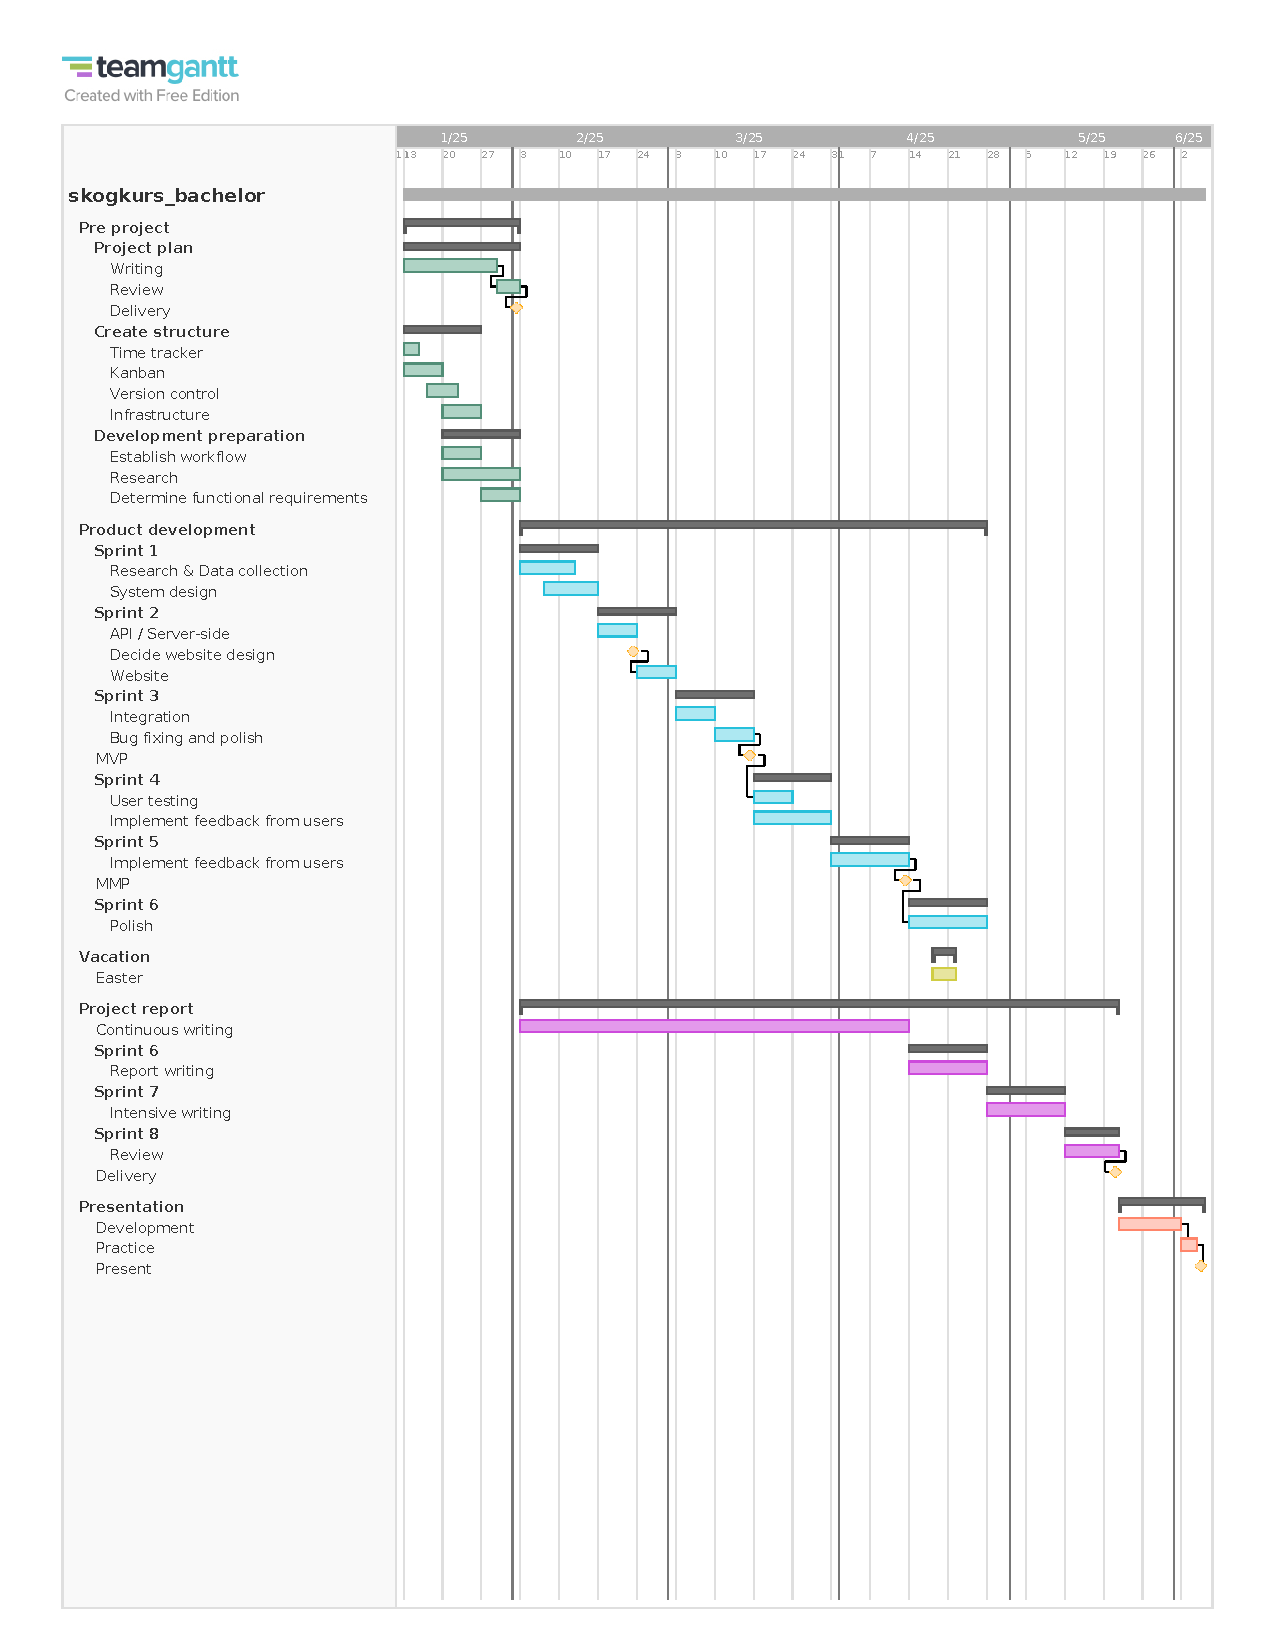
\includegraphics[width=1.0\linewidth, trim=0 60mm 0 20mm, clip]{figures/skogkurs_bachelor_gantt.pdf}
    \caption{Gantt diagram of the project}
    \label{fig:gantt_diagram}
\end{figure}

\section{Software Development Lifecycle Model}

For this project, the team needed to select an appropriate \acrfull{sdlc} model. Key factors considered in this decision included the clarity and flexibility of the requirements, team size, project timeline, product delivery goals, and prior experience \cite{sdlc_model}. 

The requirements provided by the Product Owner are intentionally ambiguous and flexible, allowing the team to prioritize the few fixed requirements upfront while iteratively refining the flexible ones over time. The team is composed of two members with similar experience levels, enabling close collaboration and effective decision-making. With a short project timeline of four months, a structure of 2-week sprints aligns perfectly with Scrum's iterative and adaptive approach, ensuring steady progress and regular opportunities for feedback. 

Given the absence of clearly defined requirements and the need for continuous collaboration with the Product Owner, the Scrum methodology was the most appropriate framework for managing the team’s workflow and project development. Traditional methodologies like Waterfall are not suitable, as they rely on fixed requirements and a linear development process, which would limit the teams flexibility \cite{waterfall_model_enwiki:1275499744}. Extreme Programming (XP), while valuable for high-collaboration environments with strict engineering practices like pair programming and test-driven development, is not fully suitable as the project does not emphasize these practices to the same extent \cite{extreme_programming}. Similarly, Lean development focuses on minimizing waste and maximizing efficiency but is less structured in terms of iterative planning, which is needed to manage evolving requirements effectively \cite{lean_programming}. By adopting Scrum, the team can iteratively refine requirements and adapt to changes throughout development \cite{sdlc_model}. To implement Scrum effectively, several key practices are integrated into our workflow \cite{scrum_guide}.

\begin{itemize}
    \item \textbf{Sprint Meetings:} The project is divided into 2-week sprints. At the start of each sprint, sprint meetings included sprint planning, reviews, and retrospectives. During the planning phase, the team selects tasks from the product backlog to form the sprint backlog for the upcoming sprint. The review phase focuses on evaluating progress and determining whether adjustments to the product backlog are needed. The goal of the retrospective phase is to identify areas for improvement in the Scrum process itself.
    \item \textbf{Daily Scrum Meetings:} Short daily meetings are conducted to discuss the progress of ongoing tasks, identify potential obstacles, and ensure alignment between team members. 
    \item \textbf{Scrum Master:} Given that the team consists of only two members, we have decided to share the role of Scrum Master. Both members are responsible for ensuring adherence to the Scrum framework and continuously working to improve team efficiency. This collaborative approach allows us to maintain flexibility while upholding Scrum principles throughout the project.
    \item \textbf{Kanban:} To complement Scrum and further enhance workflow visibility, a Kanban board is utilized to track and manage tasks on GitHub. The Kanban board consists of columns representing different stages of the workflow, such as Product Backlog, Sprint Backlog, In Progress, In Review, Done, and Discarded.
\end{itemize}

\section{Sprints}

\textcolor{orange}{Sammenlign med det som står over, ta med sprint planning, reviews og retrospective. Sprint Reviews for selve produktet, retrospectives for prossessen. Lite å snakke om på retrospektive, men var en periode med lite arbeid på bachelor på grunn av annet fag (vet ikke om det skal nevnes?). Kanskje spesifiser for enkelte sprints i hvilken iterasjon websiden er i, hvis man skal sammenligne med det som nevnes i implementation? Burde vi ta med hvordan vi divergerte fra planen?}

For more details about the sprints, the meeting minutes from each sprint meeting can be found in \autoref{appendix:sprint_meetings}.

\textcolor{orange}{legge til mer interessant tittel på sprints? ikke bare Sprint N}

\subsection*{Sprint 1}

The first sprint was primarily dedicated to project planning and initial research.  To determine the trafficability of forestry roads, we needed to identify reliable and relevant sources of map and geospatial data. In early discussions with the Product Owner, several potential sources were identified, including SeNorge, GeoNorge, NGU, and NIBIO. We also explored additional datasets from ESA and NASA, however these were ultimately found to have too coarse a resolution for our purposes, as forestry roads are densely distributed and require more detailed spatial data.

Given that none of the team members had prior experience with TypeScript, React, or OpenLayers, we allocated time to study their official documentation and familiarize ourselves with their concepts. In parallel, we created key system diagrams, including a use case diagram and a sequence diagram, to clarify system requirements and interactions. 

As the initial work progressed faster than anticipated, we moved on to designing the website. We first created a wireframe to outline the structure and layout of the user interface, which provided a clear foundation for development. We then began implementing the website in order to start testing different map layers and ensure the chosen technologies would meet the project’s functional requirements.

\subsection*{Sprint 2}

With the website development underway, we were able to implement several key map layers, including superficial deposits, frost depth, static soil moisture, historic soil moisture, and forestry roads. The historic soil moisture data was sourced from the \acrshort{esa}, but it was ultimately deemed unfit for our use, as it lacked forecast capabilities and had a coarse resolution of $25 \times 25\text{ km}$.

At this stage, the website had reached a level of functionality that allowed us to present it to the Product Owner and gather further feedback. The most significant point raised was the need to replace the ESA soil moisture layer with a more suitable, dynamic alternative. After some discussion, we decided to explore and attempt the integration of soil moisture forecast data from Open-Meteo.

\subsection*{Sprint 3}

During this sprint, we decided to prioritize the classification of forestry roads over the integration of Open-Meteo data, as trafficability assessment was considered more critical for delivering a functional prototype. We successfully implemented a function in the backend server to determine road trafficability, although it was initially based solely on frost depth data. Integrating the frost depth data proved more challenging than expected due to poor documentation of the API used to retrieve it. Further implementation details are provided later in \autoref{subsubsec:implementation:optimization:senorge}.

In parallel, we began outlining the thesis and taking notes for specific chapters to prepare for the documentation phase.

\subsection*{Sprint 4}

The main goal of this sprint was to continue improving the classification of forestry road trafficability. In addition to frost depth, we incorporated superficial deposits as a contributing factor. However, to fully utilize superficial deposits in the classification, we still needed a reliable data source for soil moisture content.

\subsection*{Sprint 5}

After implementing several of the classification factors, we needed to define specific threshold values for the classification logic. To aid in this, we held a meeting with the Product Owner. During this sprint, we also decided to switch from using Open-Meteo data to soil saturation data from SeNorge. This decision was based on SeNorge’s higher spatial resolution and our observations that its data appeared more reliable in comparison.

\textbf{The key factors identified for determining trafficability included:}

\begin{itemize}
    \item If the frost depth exceeds 10 cm, the road generally has good trafficability.
    \item In the absence of frost, soil saturation percentage is assessed. The threshold value depends on the type of superficial deposit, as different soil types vary in permeability and sensitivity to moisture.
\end{itemize}

Additionally, the Product Owner requested that transport managers be able to adjust these thresholds, as they can vary by location and may be informed by the users’ prior experience when comparing the map data. To enable this flexibility, we decided to implement a slider for threshold adjustment, moving the classification algorithm to the frontend. Further details on the implementation of the classification algorithm can be found in \autoref{subsec:implementation:website:trafficability_algorithm}.

In collaboration with our Supervisor, we also aimed to complete the first draft of the thesis for review and feedback.

\subsection*{Sprints 6–8}

The final sprints were primarily dedicated to writing the thesis and incorporating feedback from our supervisor. All suggested revisions were implemented to improve the structure and clarity of the report.

During this period, we also held two stakeholder meetings. The first involved the Product Owner and two representatives from the Norwegian Forest Owners' Federation. We presented the product and received positive feedback, particularly on its potential value to the forestry industry.

The second meeting included the Product Owner and two transport managers, where we discussed the practical applications of the system in day-to-day logistics and planning.

For further details about these meetings, see \autoref{sec:quality_assurance_user_feedback:user_testing}.

\section{Meetings}

In addition to internal sprint meetings, the team held regular meetings with both the Supervisor and the Product Owner. Weekly meetings with the Supervisor offered opportunities to ask questions, receive technical guidance, and get constructive feedback, both on the product and the written thesis.

Meetings with the Product Owner were held on an as-needed basis rather than at fixed intervals. Most of these meetings were conducted digitally via Microsoft Teams. They were particularly valuable for clarifying requirements, discussing design decisions, and showcasing progress through product demos.

Minutes from all meetings with the Supervisor and the Product Owner can be found in \autoref{appendix:meeting_minutes}.

\section{Minimum Viable Product}

A Minimum Viable Product (\acrshort{mvp}) is a concept that focuses on learning about customers with minimal effort. An \acrshort{mvp} is an early version of a product designed to test whether customers will use or buy it, often taking the form of a simple prototype, landing page, or manually operated service. The key benefit of an \acrshort{mvp} is that it allows teams to validate ideas early, minimizing wasted effort on products that may not succeed \cite{agile_alliance_mvp}. 

\textcolor{orange}{BLE IKKE NOE MMP. Skrev om under litt: user testing -> reviews med PO, fjernet "Further details about the user testing process and findings are discussed in a later chapter."}

During the development of the website, we conducted reviews with the Product Owner to gain insights into how the target audience (transport managers) would interact with the product and identify any missing features or necessary improvements. For the \acrshort{mvp}, we prioritized implementing the core functionalities users would need, as illustrated in the use case diagram in \autoref{fig:use_case_diagram}.

\section{Minimum Marketable Product}

A Minimum Marketable Product (\acrshort{mmp}) is the next step after an \Gls{mvp} in product development. While an \acrshort{mvp} focuses on testing assumptions and user preferences, an MMP includes essential features that meet customer needs, provide a good user experience, and generate business value. It is designed to launch quickly with must-have functionality, avoiding unnecessary features that add complexity without value. The MMP approach involves refining the product to only what is essential for success. Typically, teams first develop \acrshort{mvp}s to gather insights, then use these findings to build an \acrshort{mmp} ready for general release. In agile development, combining \acrshort{mvp} and \acrshort{mmp}s helps streamline product evolution while minimizing risk and unnecessary work \cite{wanner_mmp}. 

The initial plan was to conduct user testing and implement the feedback given to create a \acrshort{mmp}, but due to unforeseen circumstances this would not be created. This will be discussed later in \autoref{chap:discussion}.
